\noindent \textbf{Exercício 2} (2.5 pontos) A tabela abaixo mostra as soluções relaxadas para
todas as combinações de variáveis livres e fixas para um modelo de PLI.
O modelo visa a maximização da função objetivo, com $x_1, x_2, x_3 \in \{0, 1\}$.
Utilizar busca por profundidade (mas não pare na primeira solução inteira)
para achar a solução ótima. Dado uma relaxação $x_1' , x_2', x_3'$ , a variável $x_i$
escolhida para ramificação será aquela cujo valor $x_i'$ na solução relaxada
esteja mais próximo de 0.5; considere também que, se os ramos possíveis
forem $x_i = 0$ e $x_i = 1$, o primeiro ramo a ser explorado é aquele cujo valor
esteja mais próximo de $x_i'$ — por exemplo, dado o resultado da relaxação
$(0.3,1,0.9)$ $x_1$ será explorado primeiro, começando pelo ramo $x_1 = 0$.
Apresente o resultado na forma de uma árvore de busca, enumerando
a sequência de exploração dos nós. Além disso, apresente uma lista
descrevendo as operações realizadas em cada nó explorado (seguindo a
mesma sequência de exploração).

\begin{figure}[H]
    \centering
    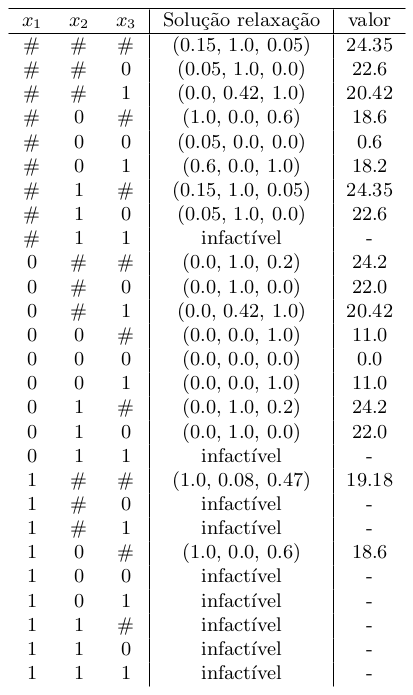
\includegraphics[scale=0.5]{table.png}
\end{figure}

\bigskip

\noindent \textbf{Solução:} A \autoref{fig:tree} apresenta a árvore resultante da busca em profundidade. Diferentemente do algoritmo original de busca em profundidade, que termina quando encontra uma solução viável, no nosso caso o algoritmo continua realizando a busca, resultando, portanto, em uma árvore.

\begin{figure}[H]
    \centering
    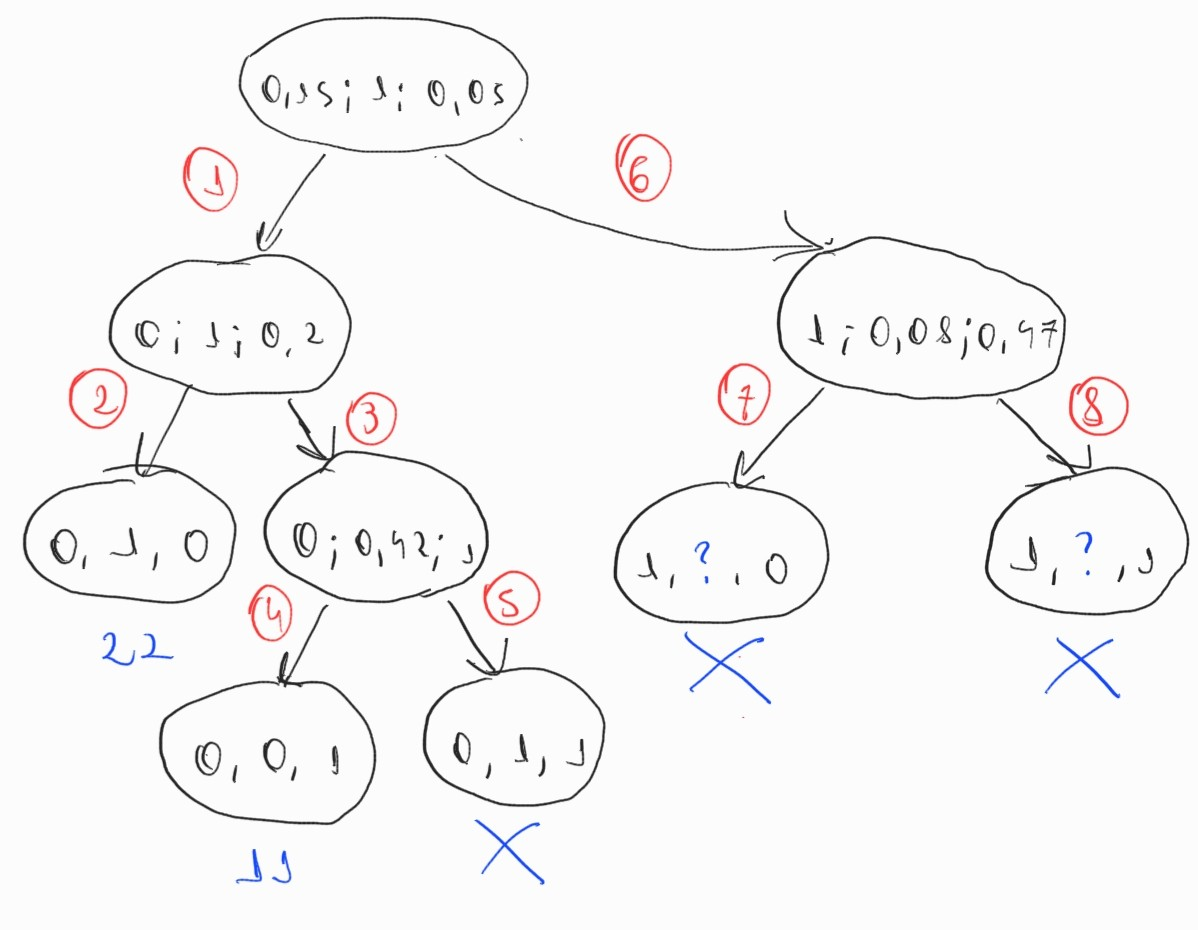
\includegraphics[width=0.8\linewidth]{tree.jpg}
    \caption{Cada nó da árvore apresenta uma solução relaxada. As setas indicam ramificações. Os números em vermelho indicam a ordem das operações (e fazem referência à \autoref{tab:list}. Os números em azul indicam o valor encontrado no nó. O X em azul indica uma solução infactível, de modo que não é mais possível seguir a partir dali.}
    \label{fig:tree}
\end{figure}

\begin{table}[H]
\centering
\caption{Lista de operações realizadas durante a busca na árvore.}
\label{tab:list}
\begin{tabular}{c|c}
\textbf{Operação} & \textbf{Ramifica} \\ \hline
1                 & $x_1$ em 0        \\ \hline
2                 & $x_3$ em 0        \\ \hline
3                 & $x_3$ em 1        \\ \hline
4                 & $x_2$ em 0        \\ \hline
5                 & $x_2$ em 1        \\ \hline
6                 & $x_1$ em 1        \\ \hline
7                 & $x_3$ em 0        \\ \hline
8                 & $x_3$ em 1       
\end{tabular}
\end{table}
